\section{Results and Discussion}

\subsection{Dataset Overview and Feature Summary}

The curated dataset comprised 321 distinct PLGA microparticle formulations drawn from 113 primary studies, representing 89 unique drugs and a total of 4{,}913 release measurements. Each formulation contributed between 5 and 48 time points (mean $\sim 15$), reflecting substantial heterogeneity in reporting density across studies. From these records, a fixed design matrix of 15 numeric covariates was constructed (Table~\ref{tab:summary_stats}).

Six variables were computed directly from drug SMILES strings using RDKit, including molecular weight, lipophilicity, topological polar surface area, hydrogen-bond counts, and rotatable bonds. Three additional drug properties were taken as reported in the source literature. The remaining six variables describe formulation or process attributes, including polymer molecular weight, LA:GA ratio, particle size, drug loading, encapsulation efficiency, and a composite hydrophilicity index.

% ============================================================
% TABLE 1: Summary Statistics
% ============================================================

\begin{table}[H]
\centering
\caption{Summary statistics of input features across 321 formulations (formulation-level means shown).}
\label{tab:summary_stats}
\small
\begin{tabular}{llrrrr}
\toprule
Feature & Source & N & Mean $\pm$ SD & Min & Max \\
\midrule
Drug MW & Drug property & 321 & 432.41 $\pm$ 232.60 & 130.08 & 1488.81 \\
Drug LogP & Drug property & 321 & 2.76 $\pm$ 2.35 & -11.55 & 9.11 \\
Drug TPSA & Drug property & 321 & 101.26 $\pm$ 96.79 & 6.48 & 701.77 \\
Polymer MW & Formulation & 321 & 37.07 $\pm$ 29.09 & 2.30 & 215.00 \\
Particle Size & Formulation & 321 & 46.04 $\pm$ 46.46 & 1.15 & 295.70 \\
Drug Loading Capacity & Formulation & 321 & 11.79 $\pm$ 9.42 & 0.02 & 61.90 \\
Drug Encapsulation Efficiency & Formulation & 321 & 67.07 $\pm$ 22.88 & 1.31 & 100.00 \\
\midrule
Peppas $n$ & Target & 318 & 0.657 $\pm$ 0.404 & 0.064 & 1.971 \\
Peppas $K$ & Target & 321 & 0.212 $\pm$ 0.190 & 0.000 & 0.866 \\
Burst$_{24h}$ & Target & 321 & 0.811 $\pm$ 0.197 & 0.032 & 1.082 \\
\bottomrule
\end{tabular}
\end{table}

Korsmeyer--Peppas parameterization was successful for the majority of formulations after restricting the fit to the sub-60\% release window and enforcing physically plausible bounds ($0 \le n \le 2$). All time axes were converted to hours before fitting, so the rate constant $K$ has units of h$^{-n}$, ensuring comparability across studies. The estimated release exponent $n$ had a mean of 0.66 (SD = 0.40), spanning regimes consistent with near-Fickian diffusion through anomalous and super-Case~II behavior. The fitted rate constant $K$ averaged 0.21 (SD = 0.19). \texttt{Burst\_24h} had a mean of 0.81 (SD = 0.20), indicating substantial early-time release in most formulations.

\FloatBarrier

% ============================================================
% 3.2  GROUPED CV
% ============================================================
\subsection{Grouped Cross-Validation Performance of the Stacked Ensemble}

Table~\ref{tab:cv_performance} summarizes grouped 10-fold cross-validation performance for the three regression targets, with \texttt{Formulation Index} used as the grouping variable to prevent within-formulation leakage. All reported metrics use the same benchmark protocol as the model comparison in Table~\ref{tab:benchmarking}. The release exponent $n$ was the most predictable target ($R^2 = 0.201$, MAE = 0.287). Prediction of $K$ was comparable ($R^2 = 0.199$), and \texttt{Burst\_24h} exhibited minimal recoverable signal ($R^2 = 0.087$).

% ============================================================
% TABLE 2: CV Performance
% ============================================================

\begin{table}[H]
\centering
\caption{Stacked ensemble cross-validation performance (grouped 10-fold, identical protocol to benchmark comparison).}
\label{tab:cv_performance}
\begin{tabular}{lcc}
\toprule
Target & $R^2$ & MAE \\
\midrule
Peppas\_n & 0.201 & 0.287 \\
Peppas\_K & 0.199 & 0.135 \\
Burst\_24h & 0.087 & 0.154 \\
\bottomrule
\end{tabular}
\end{table}

\FloatBarrier

% ============================================================
% 3.3  BENCHMARKING
% ============================================================
\subsection{Benchmarking Against Baseline Model Families}

The stacked ensemble was benchmarked against linear regression, random forest (RF), and gradient-boosted trees (XGBoost) under the same grouped cross-validation protocol (Table~\ref{tab:benchmarking}). For $n$, XGBoost achieved the highest $R^2$ (0.404), followed by RF (0.386), linear regression (0.224), and the stacked ensemble (0.201). For $K$, XGBoost again performed best ($R^2 = 0.208$). For \texttt{Burst\_24h}, all models performed poorly; linear regression yielded negative $R^2$. Because performance converged across structurally distinct model families and the objective of this study is to diagnose information limits rather than to maximize benchmark accuracy, we retain the stacked ensemble primarily to support the uncertainty proxy (Section~\ref{sec:uncertainty}, base-learner disagreement) and to test robustness of conclusions across hypothesis classes.

% ============================================================
% TABLE 3: Benchmark Comparison
% ============================================================

\begin{table}[H]
\centering
\caption{Benchmark comparison across model families under grouped 10-fold cross-validation.}
\label{tab:benchmarking}
\begin{tabular}{llcc}
\toprule
Target & Model & $R^2$ & MAE \\
\midrule
Peppas\_n & Linear & 0.224 & 0.276 \\
Peppas\_n & RandomForest & 0.386 & 0.226 \\
Peppas\_n & XGBoost & 0.404 & 0.226 \\
Peppas\_n & StackedEnsemble & 0.201 & 0.287 \\
\midrule
Peppas\_K & Linear & 0.114 & 0.137 \\
Peppas\_K & RandomForest & 0.141 & 0.119 \\
Peppas\_K & XGBoost & 0.208 & 0.117 \\
Peppas\_K & StackedEnsemble & 0.199 & 0.135 \\
\midrule
Burst\_24h & Linear & -0.038 & 0.159 \\
Burst\_24h & RandomForest & 0.074 & 0.131 \\
Burst\_24h & XGBoost & 0.066 & 0.134 \\
Burst\_24h & StackedEnsemble & 0.087 & 0.154 \\
\bottomrule
\end{tabular}
\end{table}

\begin{figure}[H]
\centering
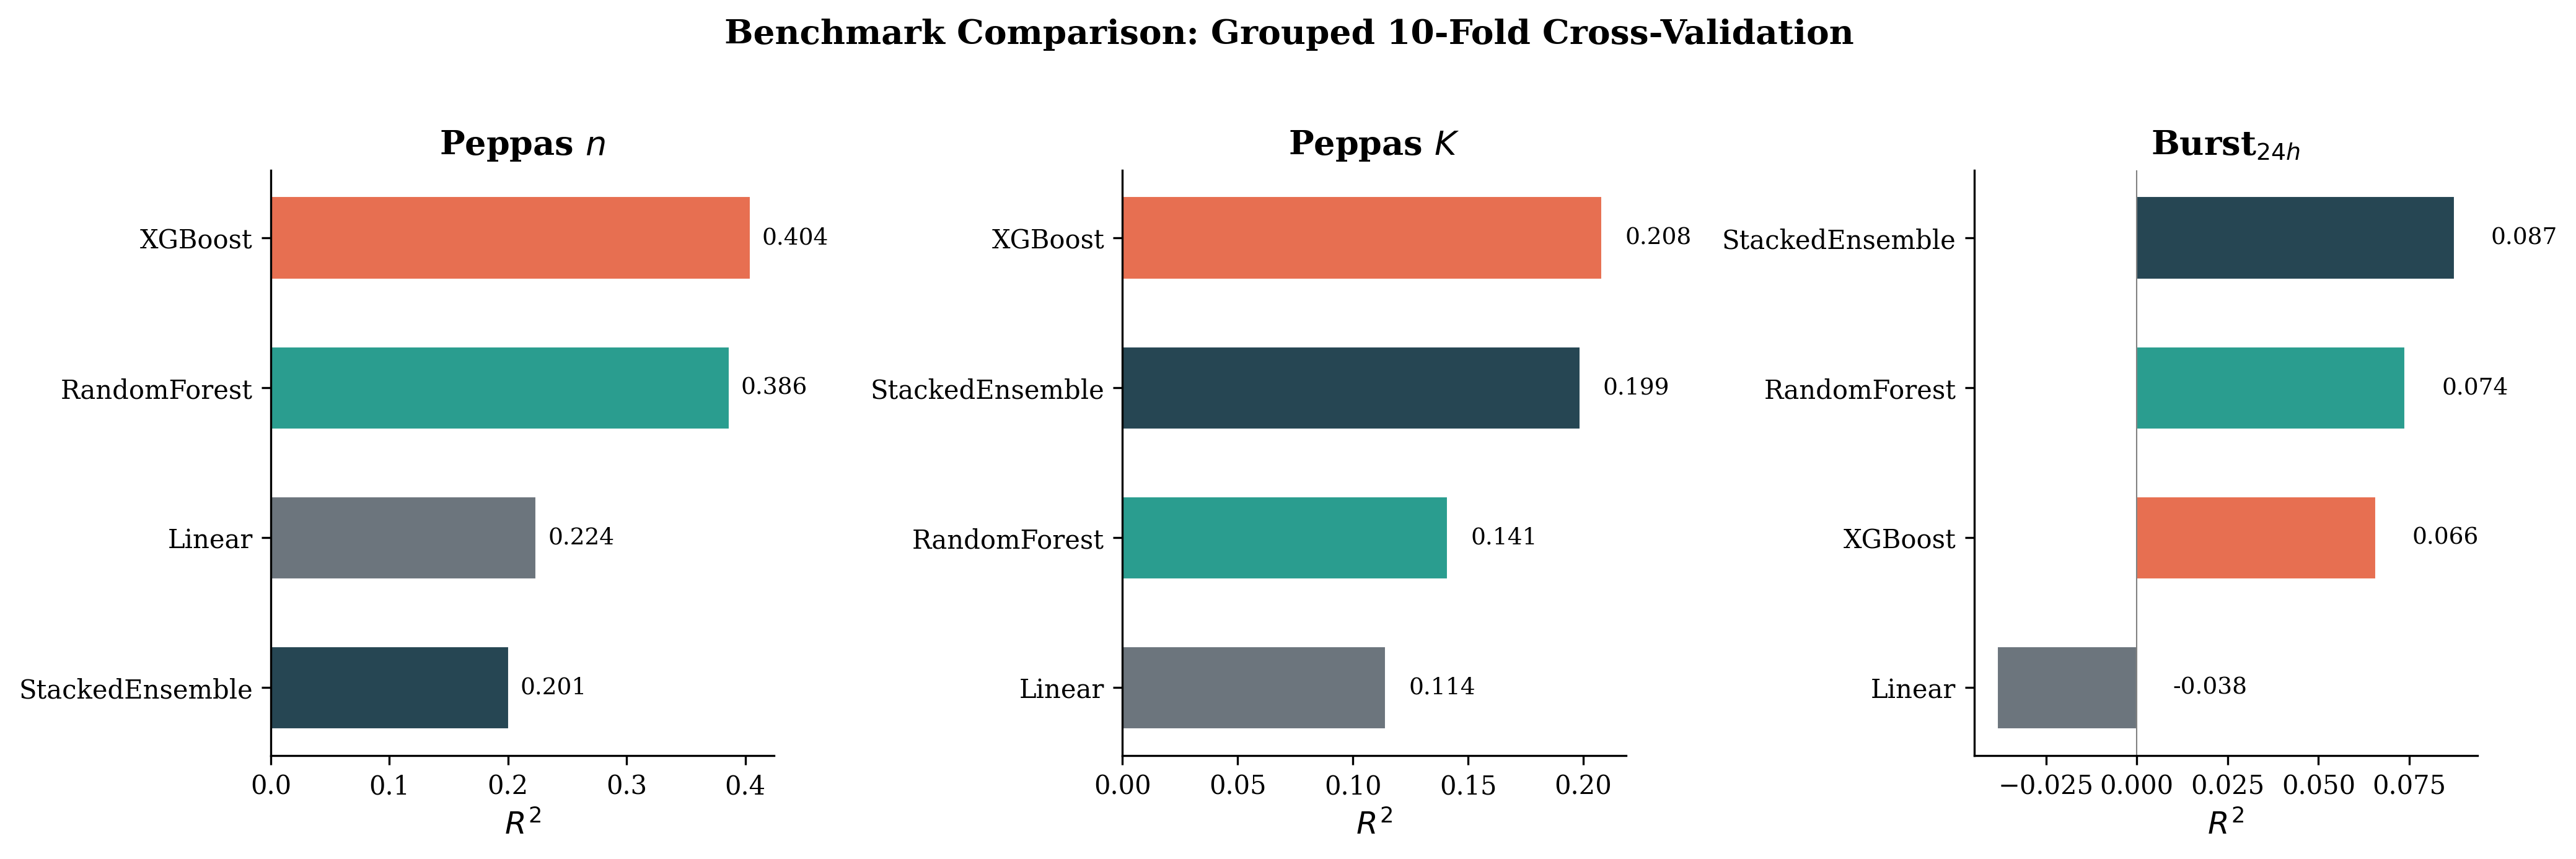
\includegraphics[width=\linewidth]{figures/fig1_benchmark_bar}
\caption{Benchmarking results for the release exponent $n$ and rate constant $K$ under grouped cross-validation.}
\label{fig:bench_bar}
\end{figure}

\FloatBarrier

% ============================================================
% 3.4  FEATURE IMPORTANCE
% ============================================================
\subsection{Feature Importance}

Feature importance for prediction of $n$ is summarized in Table~\ref{tab:feature_importance}. Polymer molecular weight contributed the largest share of importance (27.7\%), followed by drug molecular weight (13.0\%) and MolLogP (11.8\%).

% ============================================================
% TABLE 4: Feature Importance
% ============================================================

\begin{table}[H]
\centering
\caption{Features contributing $>$5\% importance for prediction of release exponent $n$ (Random Forest).}
\label{tab:feature_importance}
\begin{tabular}{lc}
\toprule
Feature & Importance (\%) \\
\midrule
Polymer MW & 27.7 \\
Drug MW & 13.0 \\
MolLogP & 11.8 \\
LA/GA & 6.1 \\
Hydrophilicity Index & 5.9 \\
Encapsulation Eff. & 5.3 \\
\bottomrule
\end{tabular}
\end{table}

\begin{figure}[H]
\centering
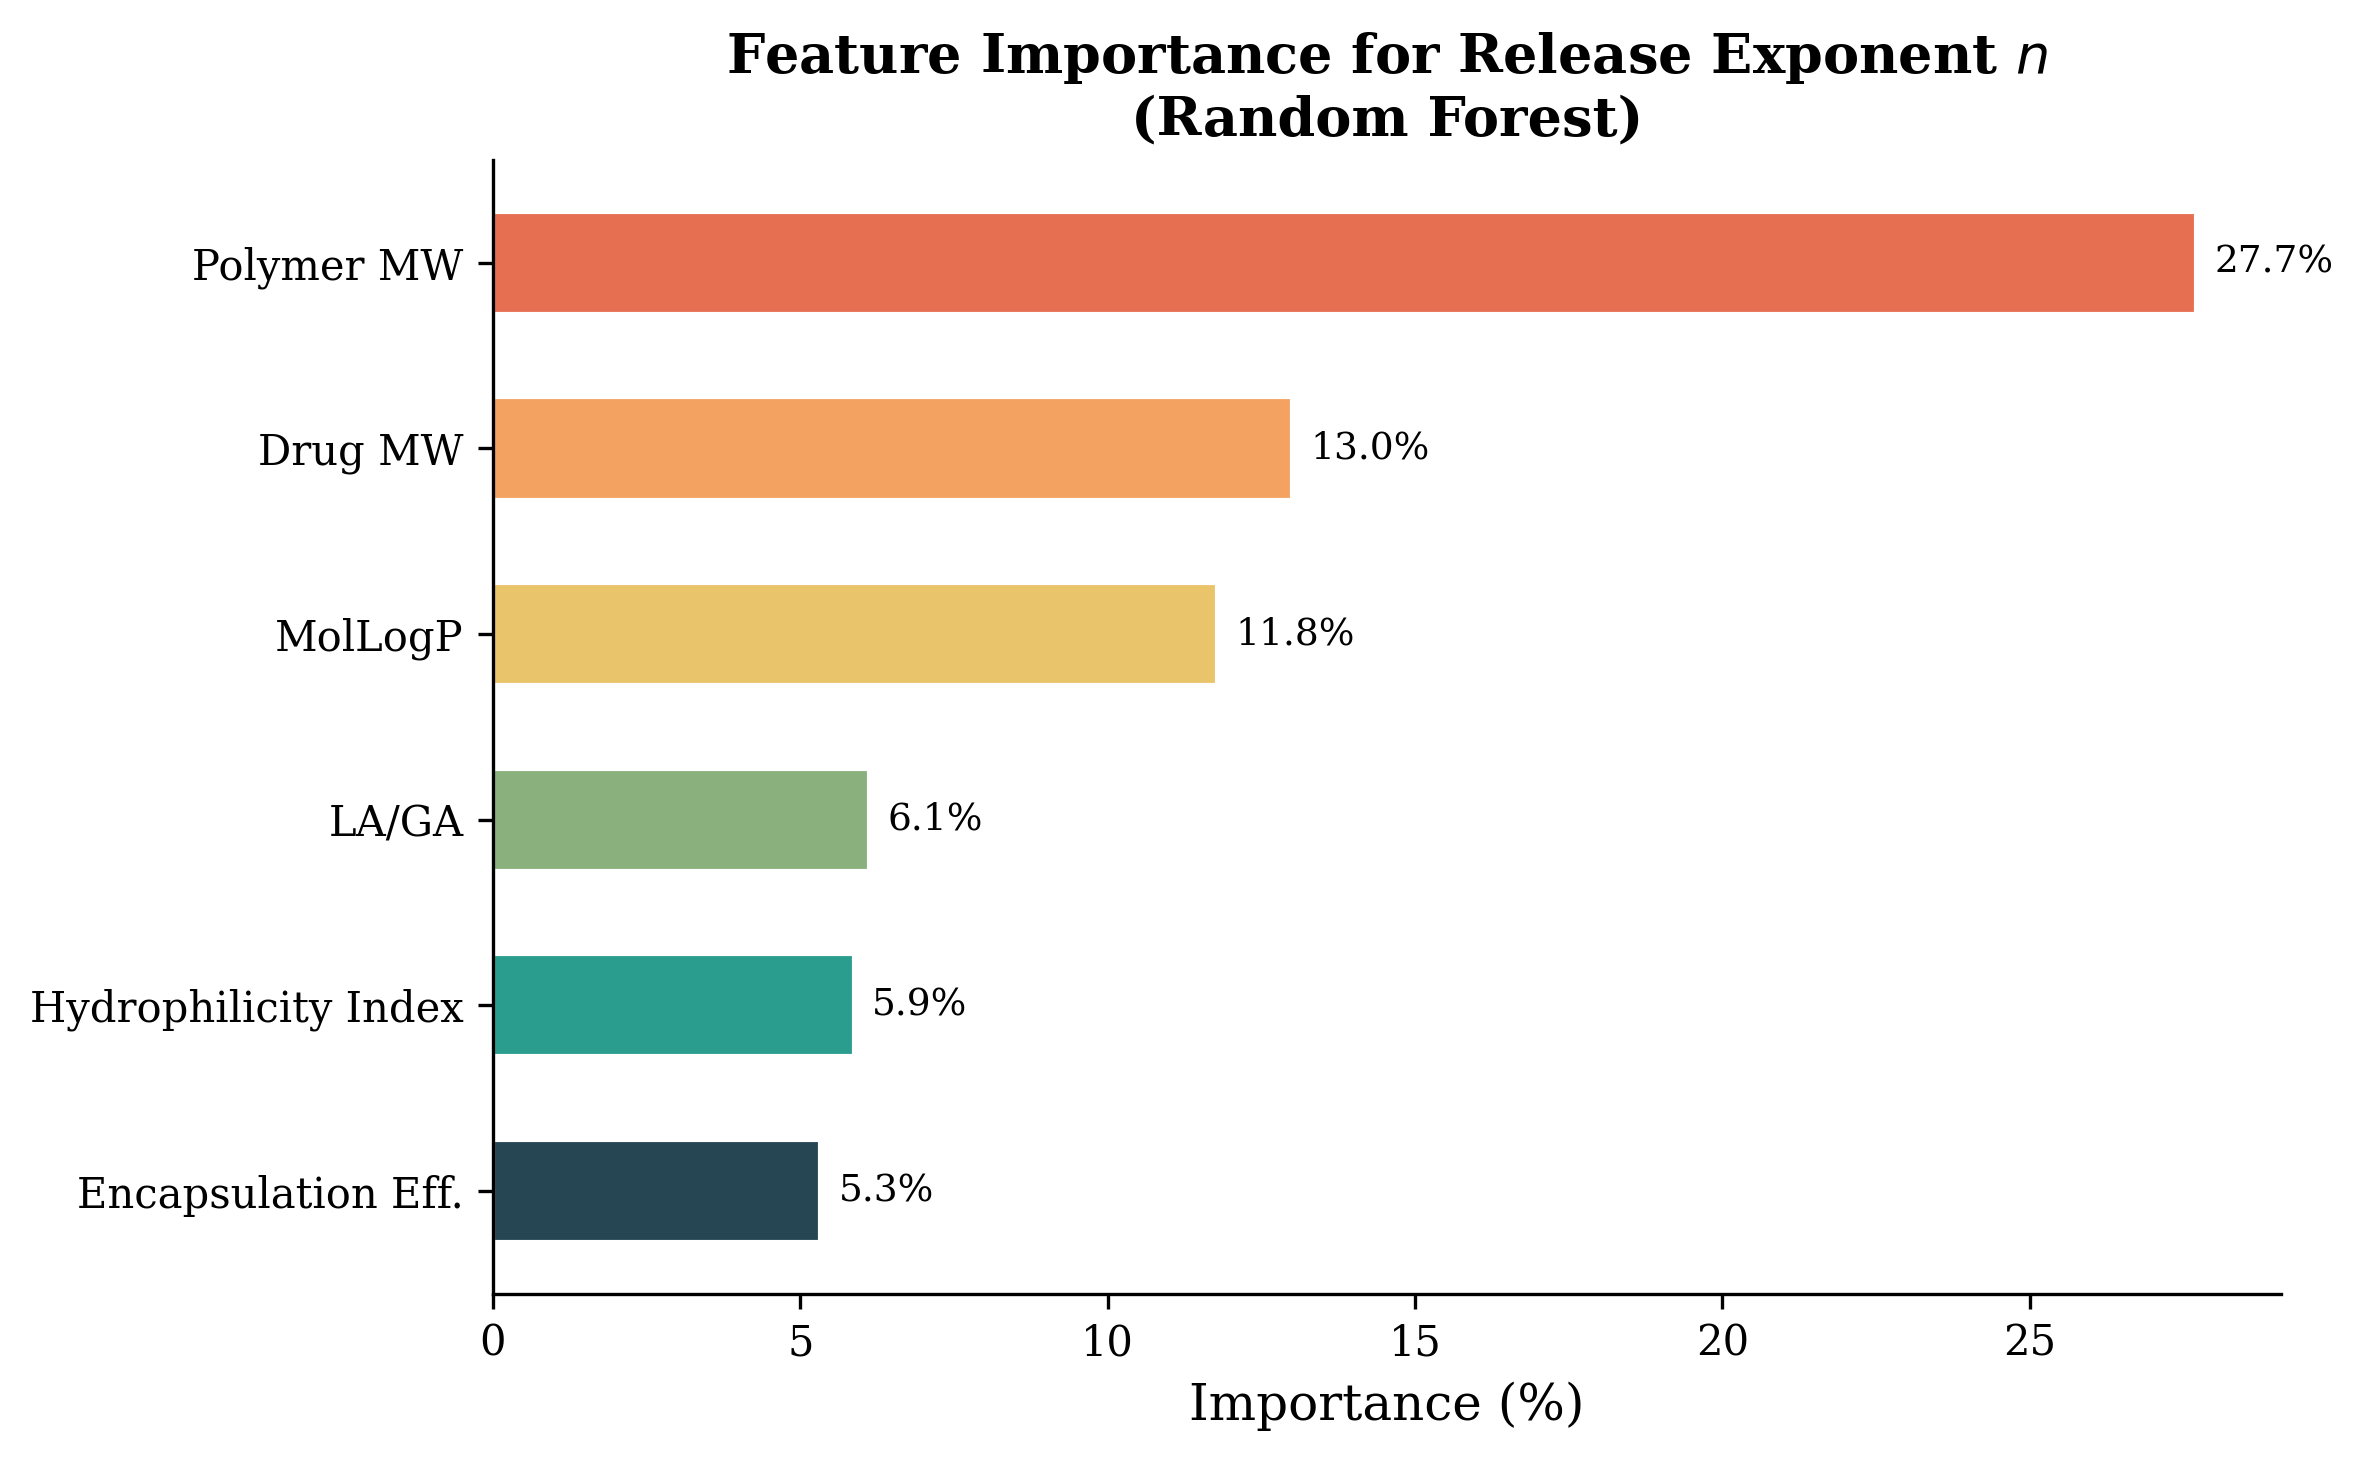
\includegraphics[width=\linewidth]{figures/fig2_feature_importance}
\caption{Top feature importances for predicting the release exponent $n$.}
\label{fig:feature_imp}
\end{figure}

\FloatBarrier

% ============================================================
% 3.5  PREDICTED VS ACTUAL
% ============================================================
\subsection{Predicted Versus Actual: Release Exponent $n$}

Predicted values for $n$ captured the overall trend but exhibited reduced dispersion relative to experimental observations. Observed $n$ values ranged from approximately 0.1 to above 1.5, whereas predictions clustered more tightly around the mean (predicted mean = 0.69, SD = 0.17 versus observed mean = 0.67, SD = 0.41).

\begin{figure}[H]
\centering
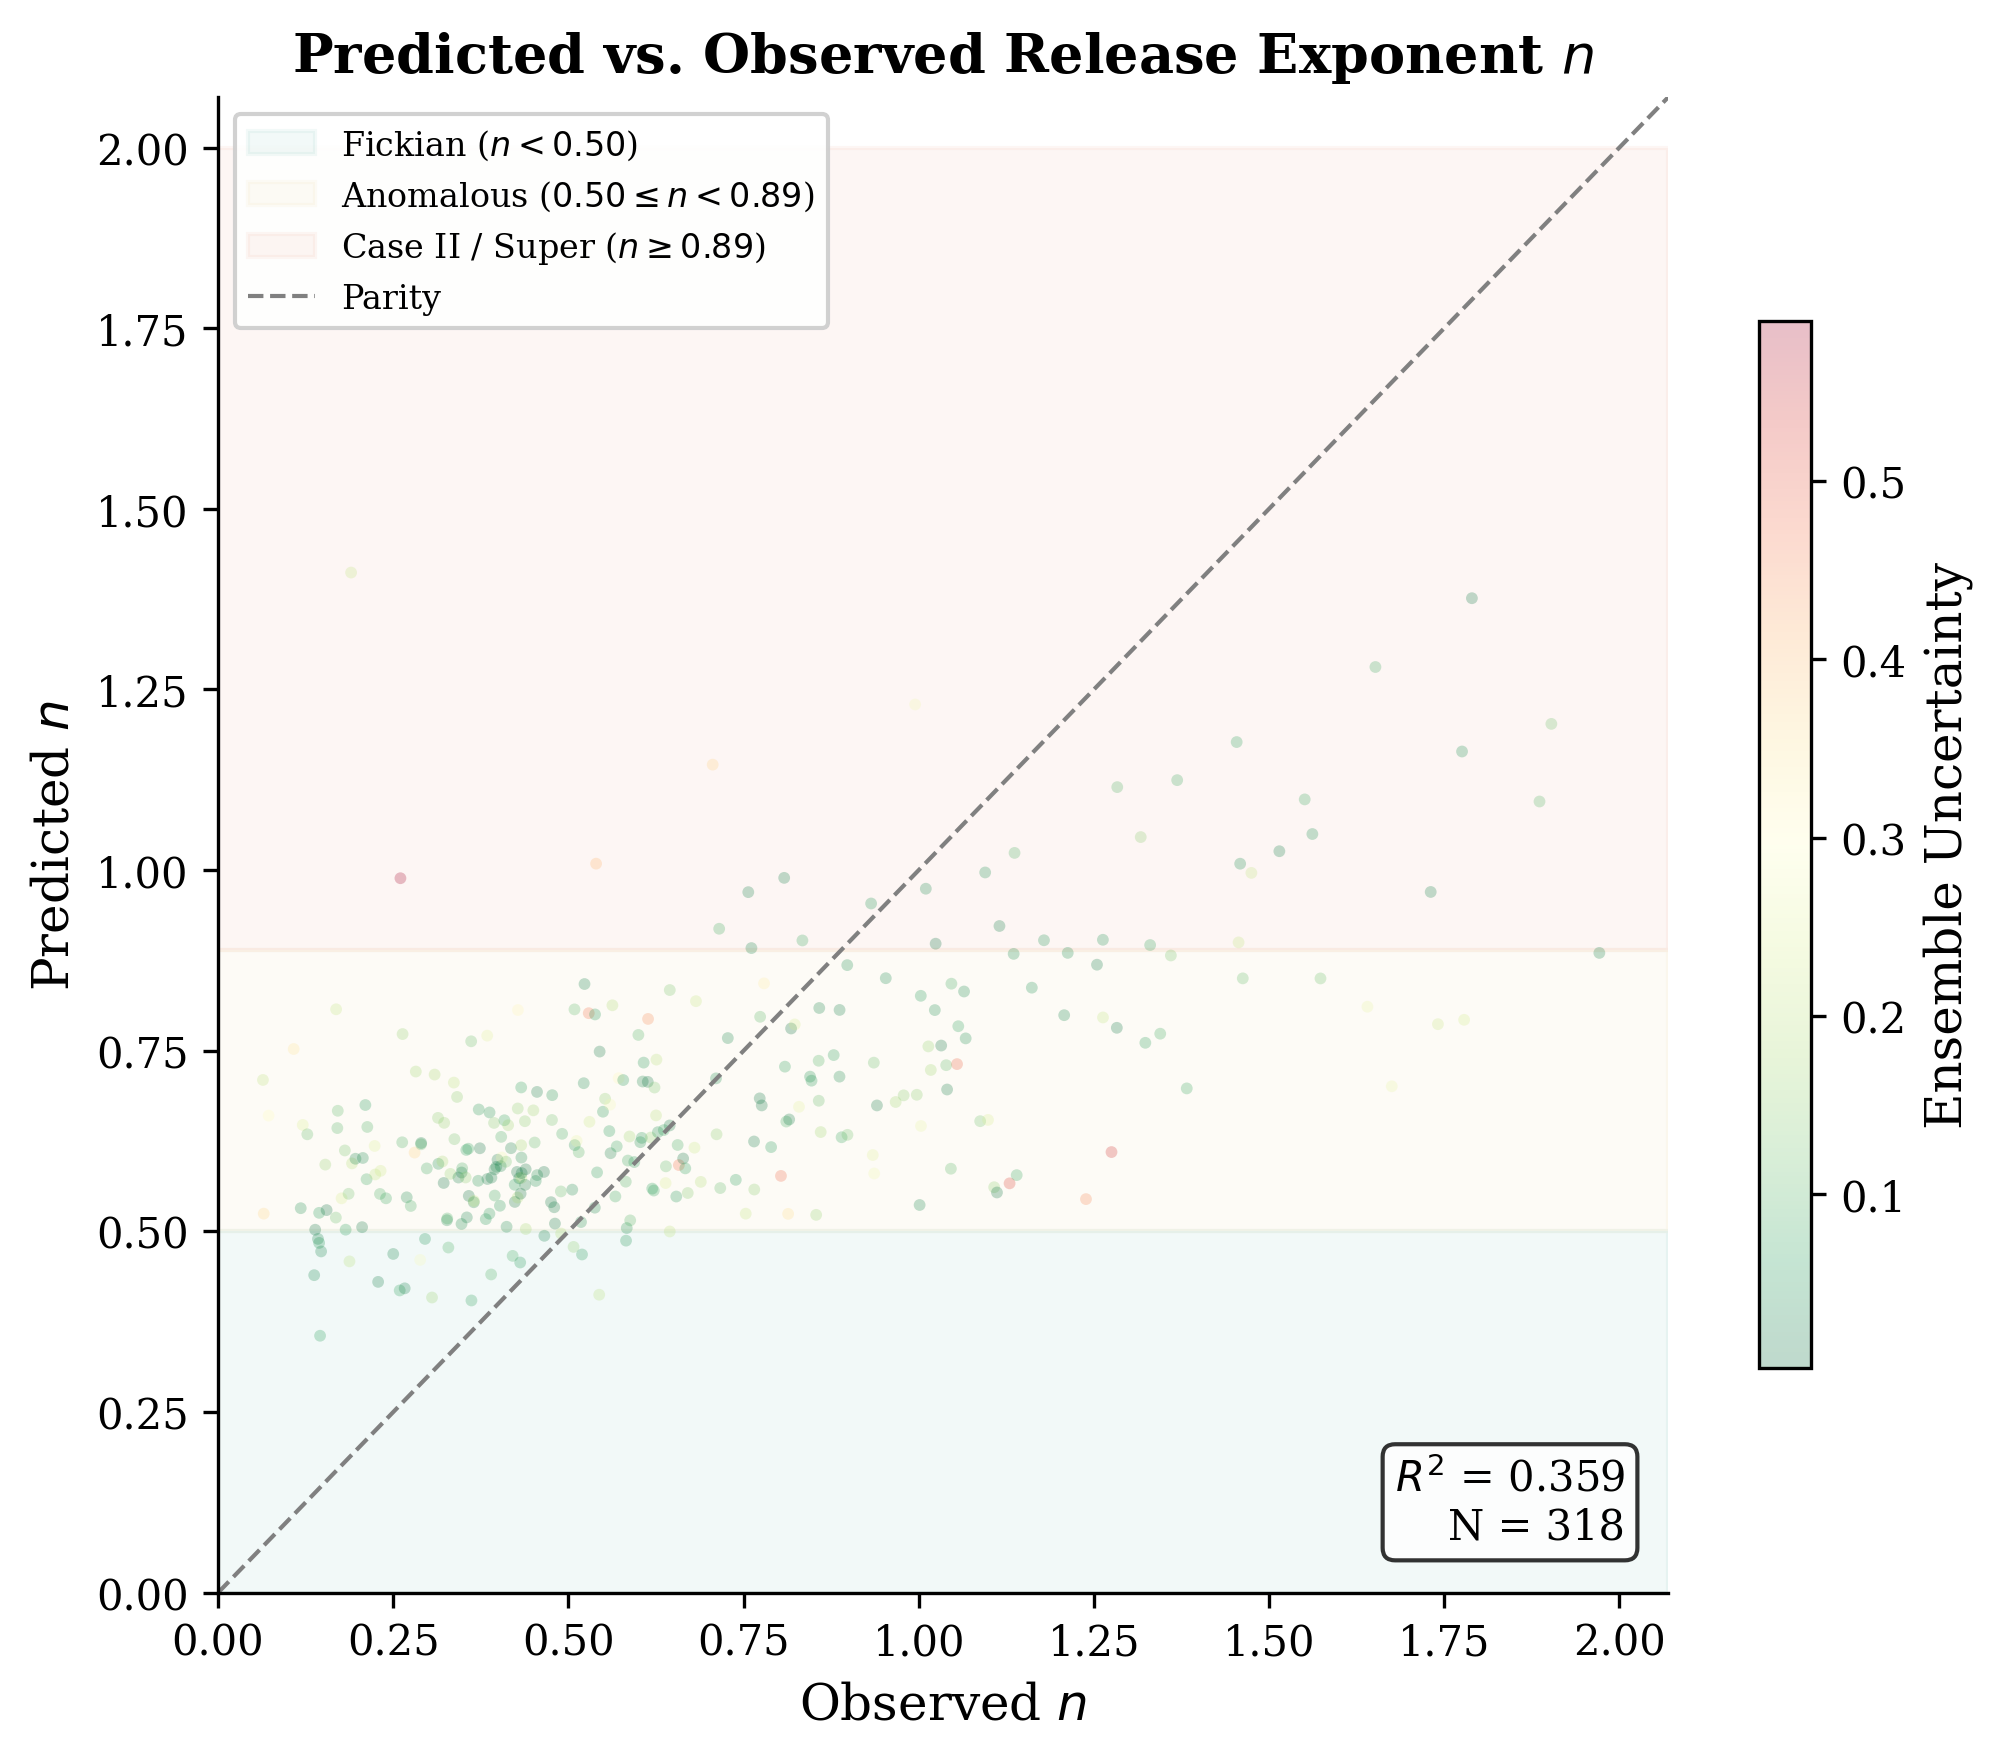
\includegraphics[width=\linewidth]{figures/fig3_pred_vs_actual_n}
\caption{Predicted versus observed release exponent $n$ (grouped cross-validation). The dashed diagonal indicates parity.}
\label{fig:pred_actual_n}
\end{figure}

\FloatBarrier

% ============================================================
% 3.6  BURST RELEASE — REFRAMED AS DIAGNOSTIC FINDING
% ============================================================
\subsection{Burst Release: Regression and Classification}

Burst release at 24 hours was the least predictable regression target ($R^2 = 0.087$, MAE = 0.154). For the complementary classification task, formulations were binned into three burst-risk classes: low burst ($< 10\%$), intermediate (10--40\%), and high burst ($\ge 40\%$). At the formulation level (321 unique formulations), the distribution was highly skewed: 305 formulations (95.0\%) were high burst, 14 (4.4\%) were intermediate, and 2 (0.6\%) were low burst.

This distribution is itself a diagnostic finding about the published record, not a model failure. The literature as compiled reflects the typical outcome of PLGA microparticles produced under standard single or double emulsion-solvent evaporation conditions: substantial early-time release is the norm. Low-burst formulations are known to depend on microstructure-level variables---internal porosity, surface drug adsorption, solvent removal kinetics, and washing/post-processing conditions---that are rarely reported in sufficient detail to support quantitative modeling \citep{Yoo2020, Fredenberg2011}. Consequently, the extreme class imbalance (95.0\% high burst at the formulation level) renders standard classification uninformative: a trivial majority-class baseline achieves 95.0\% accuracy without learning any formulation--property relationship.

\begin{figure}[H]
\centering
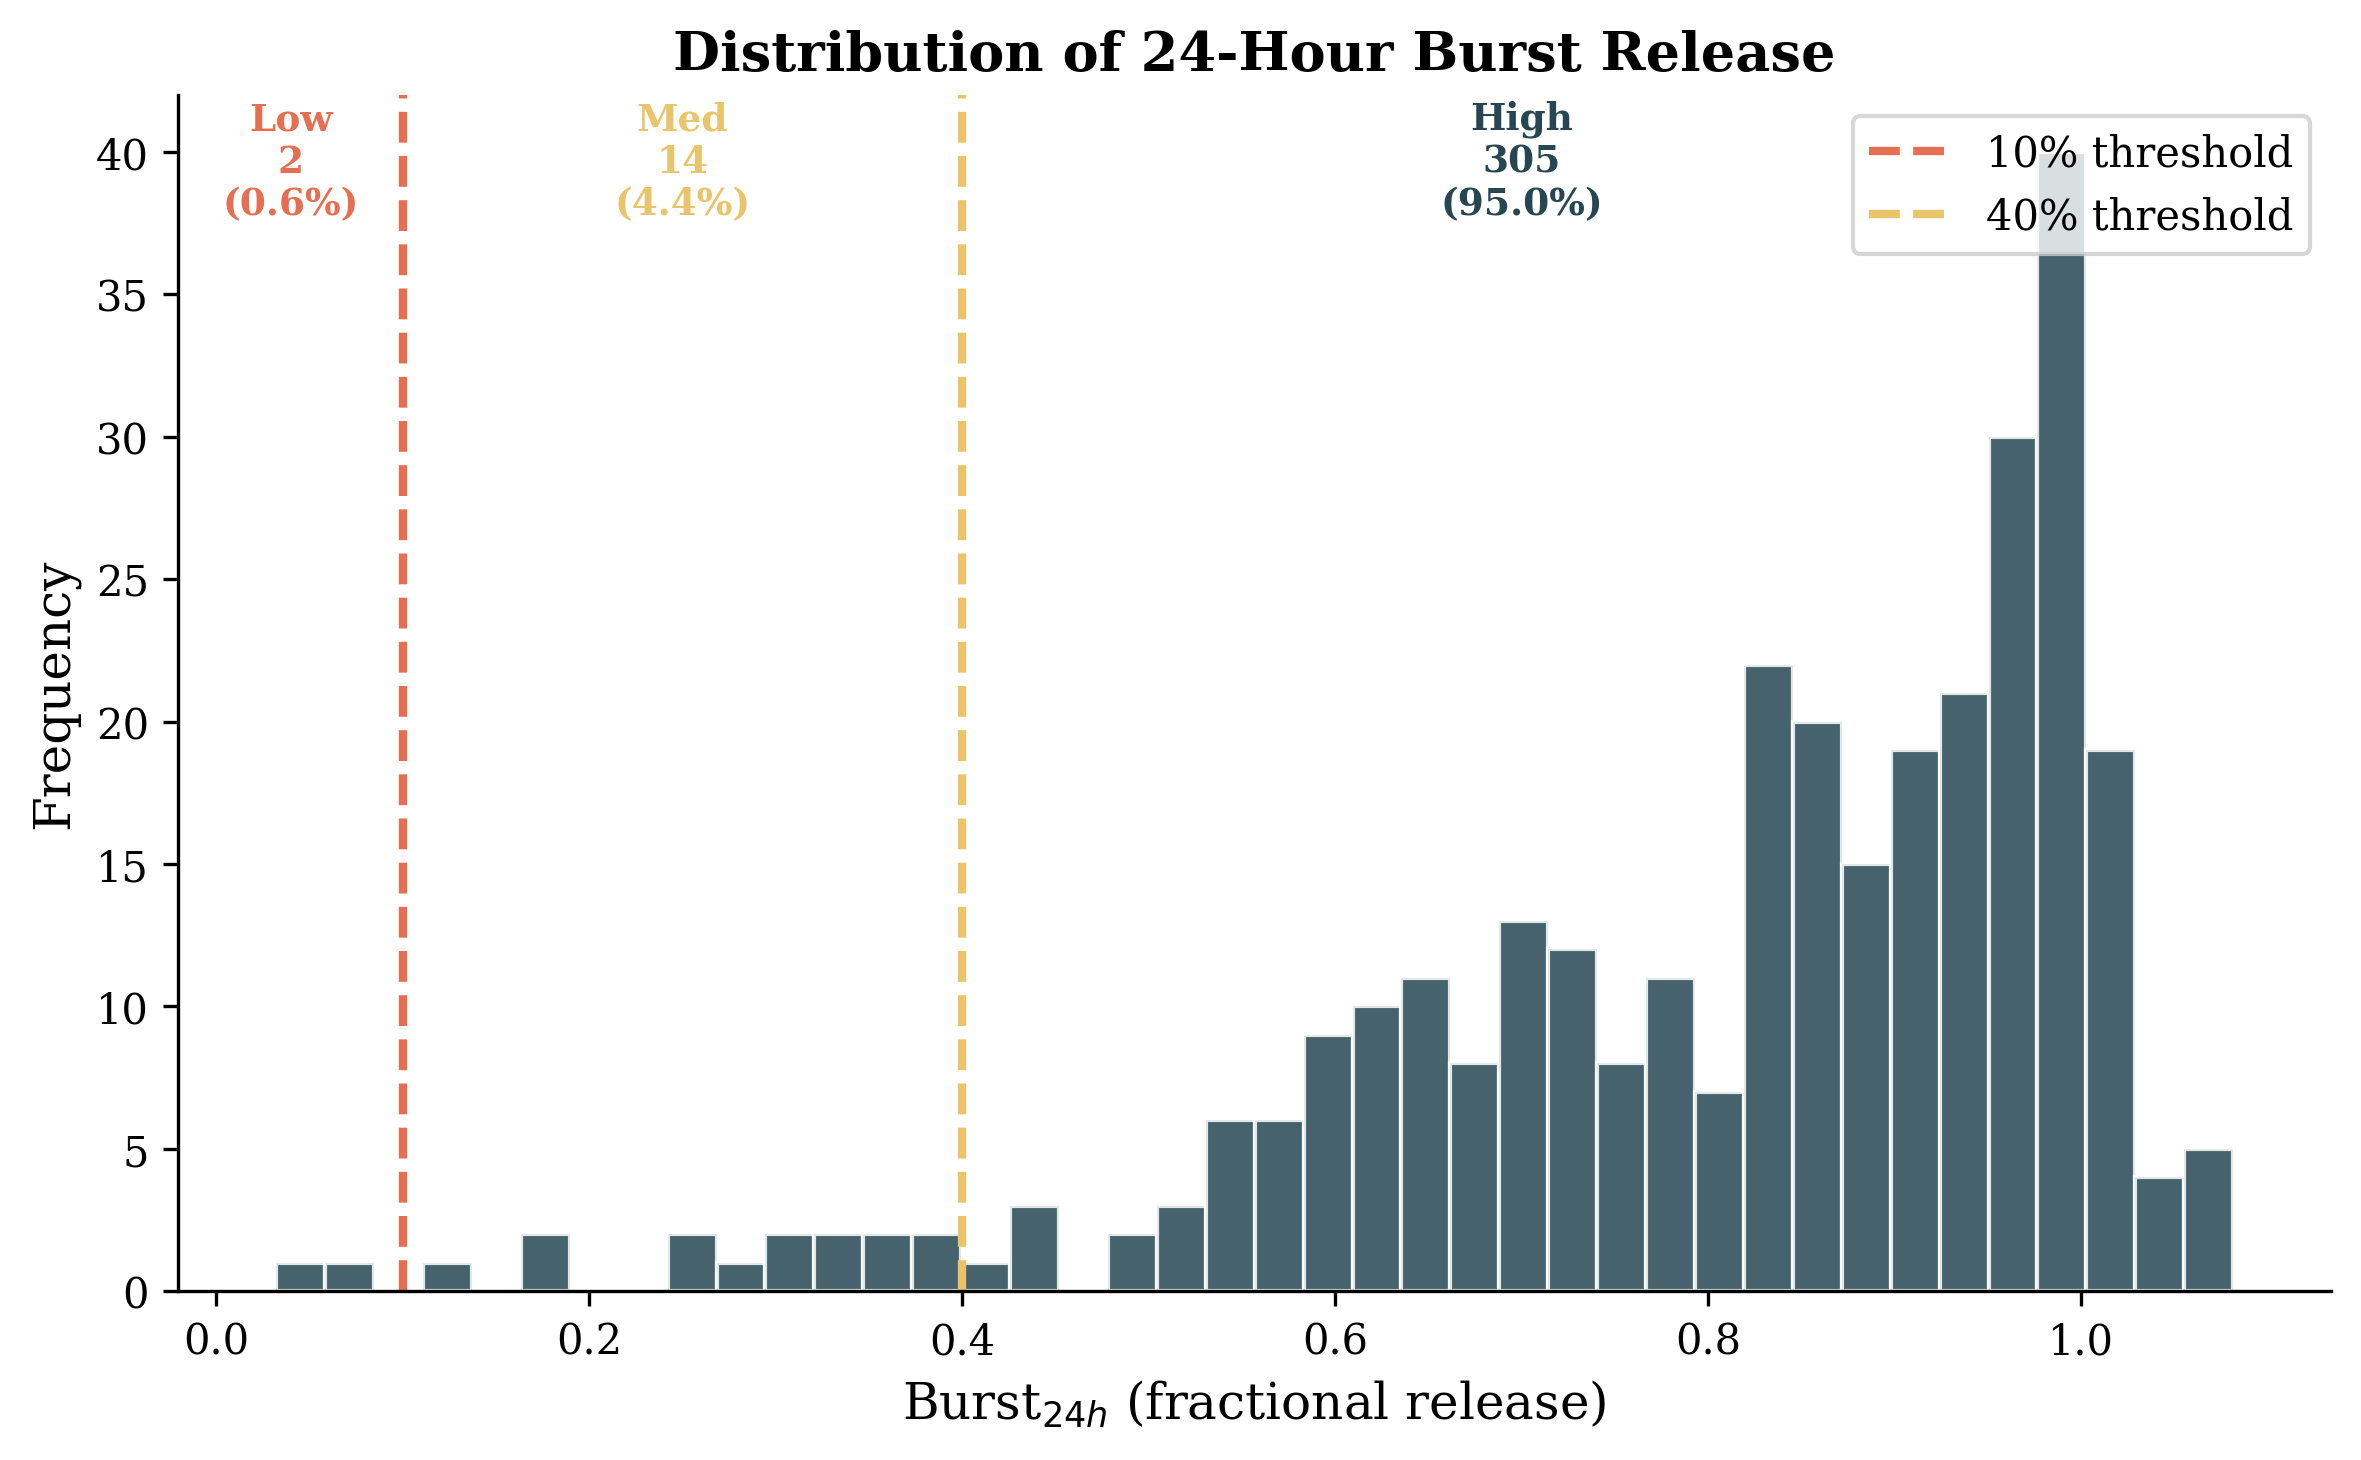
\includegraphics[width=\linewidth]{figures/fig4_burst_histogram}
\caption{Distribution of 24-hour burst release (\texttt{Burst\_24h}) with classification thresholds at 10\% and 40\%.  The extreme right skew (93\% high-burst class) reflects the dominance of standard emulsion-based formulations in the published literature and the absence of process-level variables needed to discriminate low-burst regimes.}
\label{fig:burst_hist}
\end{figure}

The confusion matrix (Table~\ref{tab:confusion_matrix}) confirmed that the model predicted only the majority class across all folds, yielding zero precision and recall for minority classes and a macro-F1 of 0.33. Under this distribution, any classifier that attempts to predict minority classes will be heavily penalized under standard metrics, rendering macro-F1 a reflection of dataset imbalance rather than model discrimination capacity. Standard remediation strategies---synthetic oversampling (SMOTE), cost-sensitive loss weighting, or ordinal regression---were considered but deliberately not applied. At a 95:4:1 class ratio with only 15 input features, synthetic minority generation would manufacture decision boundaries in sparsely populated regions of the feature space, producing misleadingly optimistic minority-class recall without genuine discriminative signal; cost-sensitive weighting faces the same fundamental limitation when the minority class lacks separability in the available covariate space. The degeneracy is diagnostic: it reflects the absence from the literature of the process-level covariates (solvent removal rate, stirring/homogenization conditions, internal porosity) that would be needed to distinguish low-burst from high-burst formulations (Section~\ref{sec:reporting_gaps}, Table~\ref{tab:reporting_gaps}). The near-absence of low-burst formulations in the published record is itself a reporting bias that hinders the development and validation of formulation strategies yielding more controlled, clinically desirable release profiles. Until the literature systematically reports these process-level drivers, burst classification from compositional covariates alone will remain degenerate.

% ============================================================
% TABLE 6: Confusion Matrix
% ============================================================

\begin{table}[H]
\centering
\caption{Confusion matrix for three-class burst-risk classification (321 formulations). Macro-F1 = 0.33.}
\label{tab:confusion_matrix}
\begin{tabular}{lccc|c}
\toprule
 & \multicolumn{3}{c}{Predicted} & \\
\cmidrule(lr){2-4}
Actual & Low & Med & High & Recall \\
\midrule
Low ($<$10\%) & 0 & 0 & 2 & 0.00 \\
Med (10--40\%) & 0 & 0 & 14 & 0.00 \\
High ($\geq$40\%) & 0 & 0 & 305 & 1.00 \\
\midrule
Precision & 0.00 & 0.00 & 0.95 & \\
\bottomrule
\end{tabular}
\end{table}

\FloatBarrier

% ============================================================
% 3.7  APPLICABILITY DOMAIN — EXPANDED WITH ISLAND CHARACTERIZATION
% ============================================================
\subsection{Applicability Domain Analysis}

Applicability-domain (AD) analysis was performed using leverage-based Williams plots, with warning leverage threshold $h^* = 3p/N$, where $p = 15$ is the number of features and $N$ is the number of unique formulations (the correct unit of analysis, since all targets are formulation-level quantities) \citep{Eriksson2003}. At $N = 321$ (or 318 for \texttt{Peppas\_n}, which had three formulations excluded during fitting), $h^*$ ranges from 0.141 to 0.142. Table~\ref{tab:ad_results} reports the results.

With formulation-level $N$, the warning leverage threshold $h^*$ is approximately 15$\times$ larger than the value obtained when timepoint rows are erroneously used ($h^* \approx 0.009$ at $N = 4{,}913$). Consequently, all 321 formulations fall below the warning leverage for every target---no high-leverage outliers are identified. This result eliminates the previously reported ``island of predictability,'' which was an artifact of the inflated denominator and correspondingly deflated threshold. The leverage values themselves (computed from the scaled design matrix) remain valid; what changes is the threshold against which they are compared. The disappearance of the island underscores that the original analysis was sensitive to a unit-of-analysis error: formulation-level targets (\textit{n}, \textit{K}, Burst$_{24h}$) must be analyzed at the formulation level, not duplicated across timepoints.

% ============================================================
% TABLE 5: AD Results
% ============================================================

\begin{table}[H]
\centering
\caption{Applicability-domain analysis: formulation-level leverage with $h^* = 3p/N$ where $N$ is the number of unique formulations.}
\label{tab:ad_results}
\begin{tabular}{llcccc}
\toprule
Target & Region & Count & $R^2$ & MAE & $h^*$ \\
\midrule
Peppas\_n & In-domain & 318 & 0.359 & 0.256 & 0.142 \\
 & High-leverage & 0 & --- & --- & \\
\midrule
Peppas\_K & In-domain & 321 & 0.171 & 0.137 & 0.140 \\
 & High-leverage & 0 & --- & --- & \\
\midrule
Burst\_24h & In-domain & 321 & 0.023 & 0.153 & 0.140 \\
 & High-leverage & 0 & --- & --- & \\
\bottomrule
\end{tabular}
\end{table}

\begin{figure}[H]
\centering
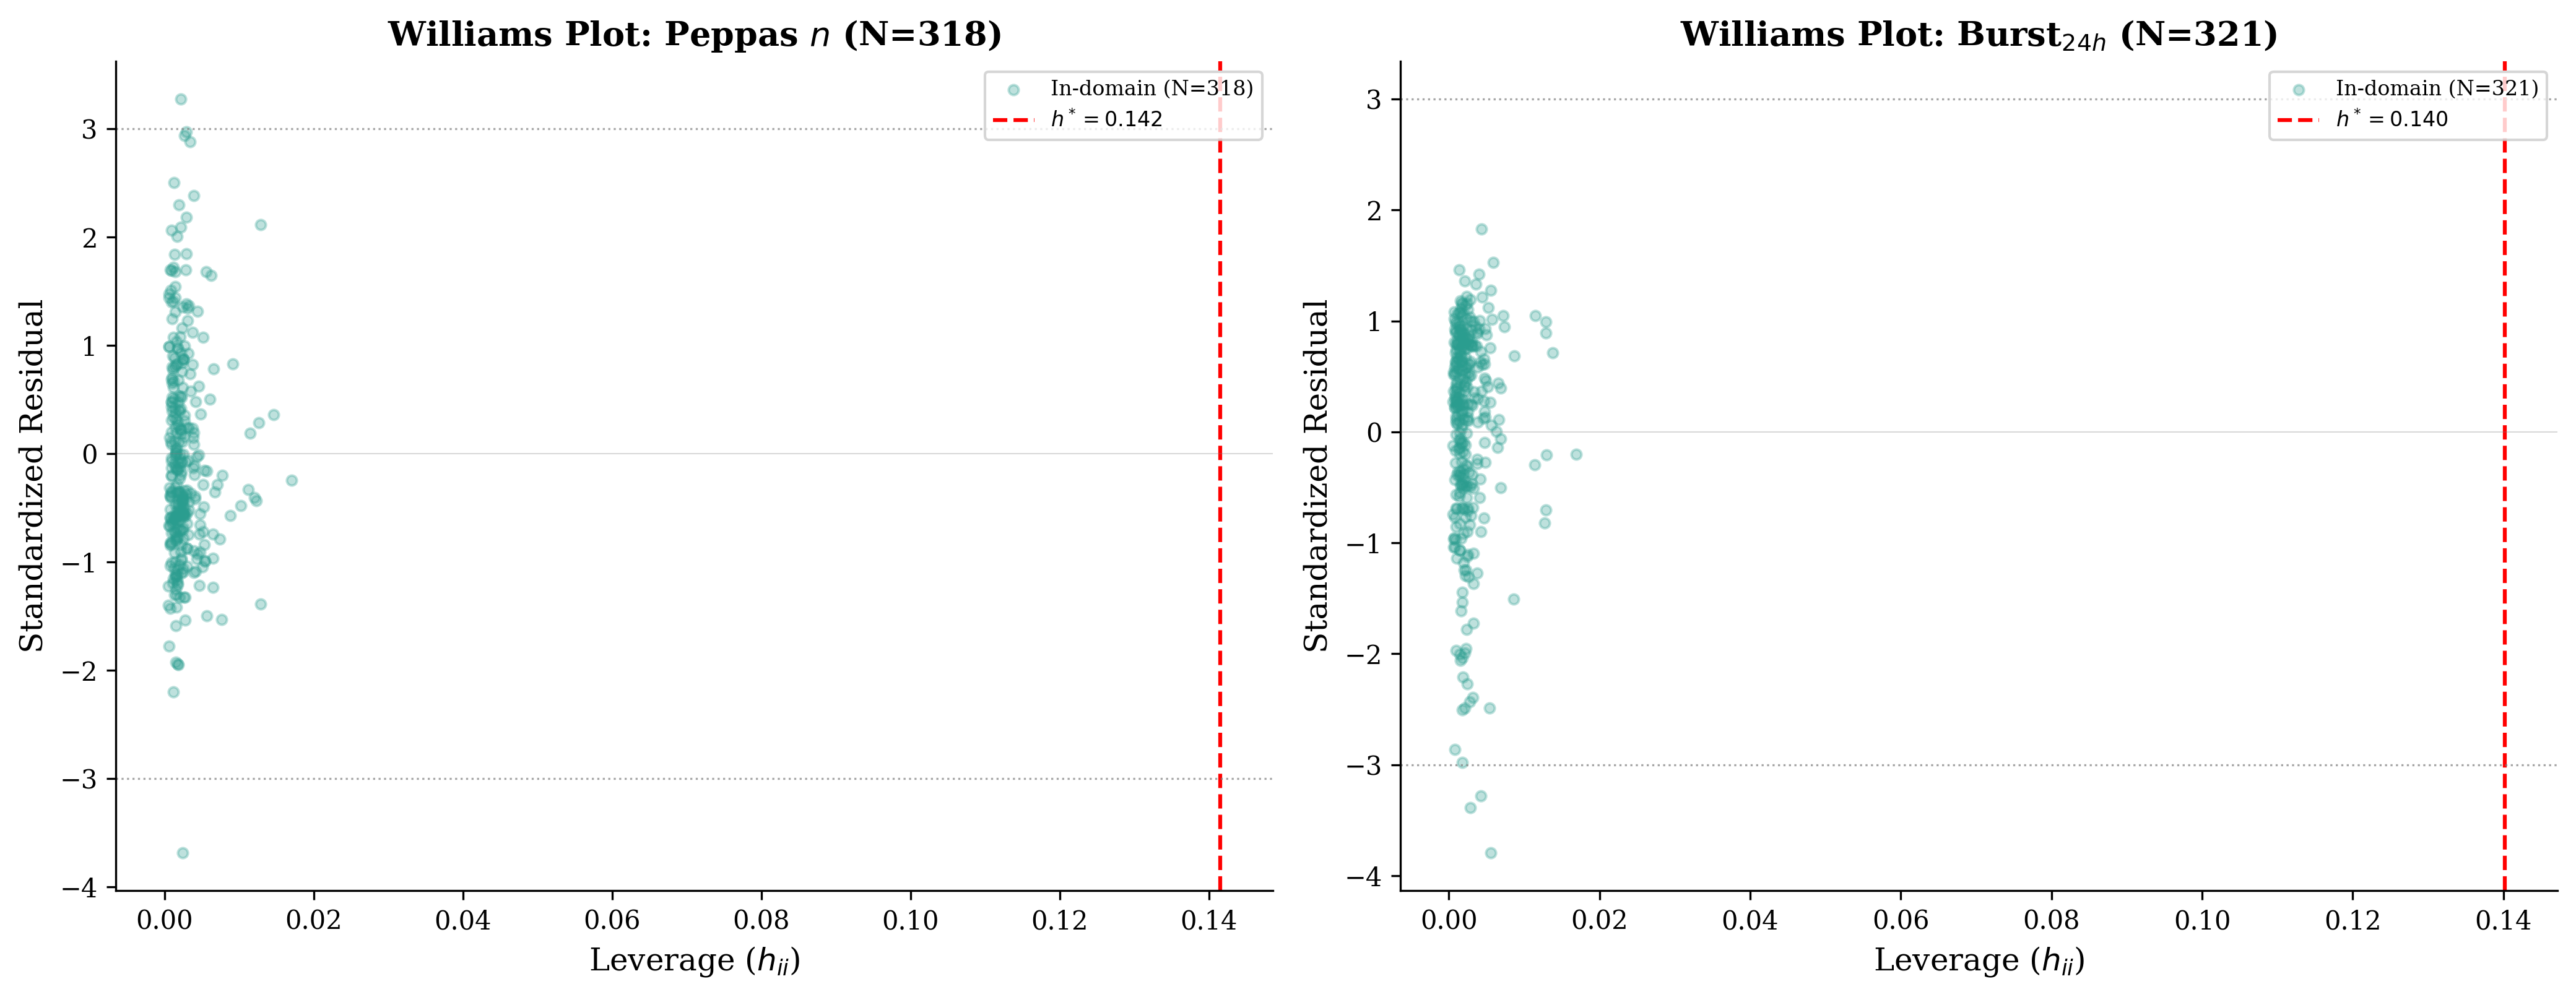
\includegraphics[width=\linewidth]{figures/fig5_williams_plot}
\caption{Williams plot for applicability-domain analysis. The vertical boundary corresponds to the warning leverage threshold $h^*$.}
\label{fig:williams}
\end{figure}

\begin{figure}[H]
\centering
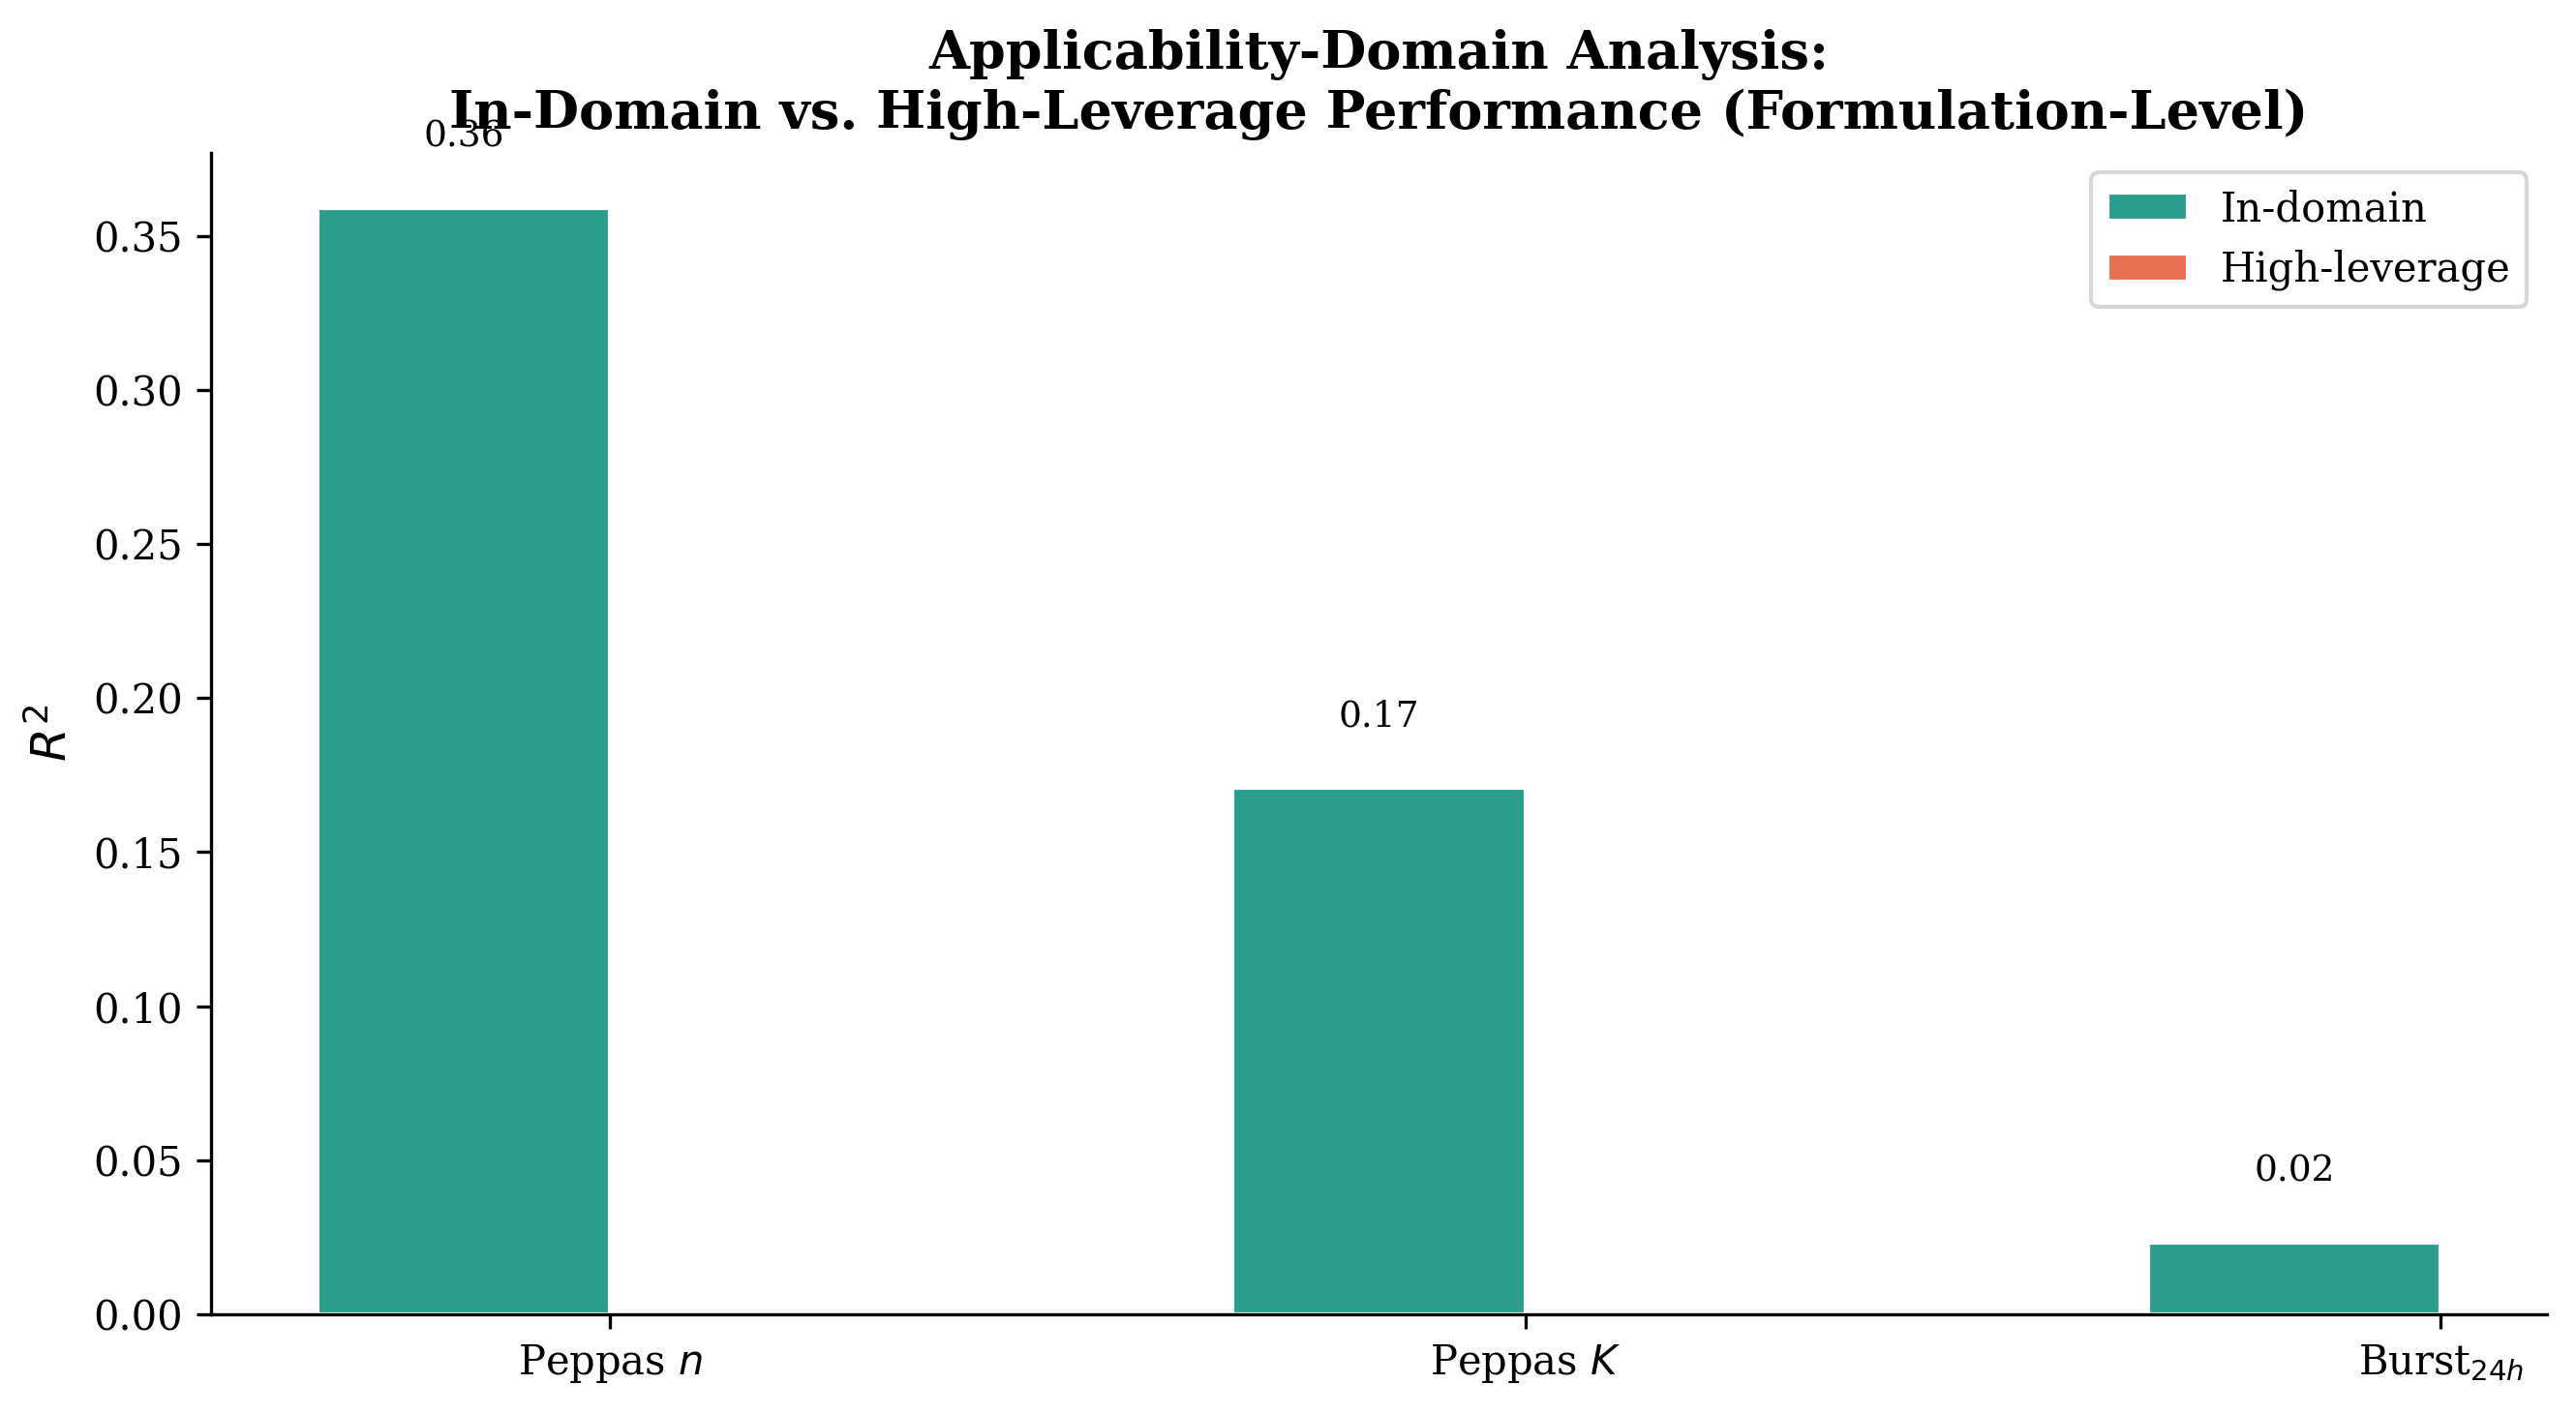
\includegraphics[width=\linewidth]{figures/fig6_ad_paradox}
\caption{Applicability-domain analysis: formulation-level $R^2$ for in-domain formulations. With the corrected threshold ($h^* \approx 0.14$), all formulations fall within the applicability domain.}
\label{fig:ad_bar}
\end{figure}

\paragraph{Note on previously reported ``island of predictability.''}
An earlier version of this analysis used the total number of timepoint rows ($N = 4{,}913$) rather than the number of unique formulations ($N = 321$) when computing the warning leverage threshold, yielding $h^* \approx 0.009$. Under that erroneously low threshold, 117 timepoint rows (corresponding to 11 formulations) exceeded $h^*$ and appeared to form a high-leverage ``island'' with elevated $R^2$. When the threshold is correctly computed at the formulation level ($h^* \approx 0.14$), no formulations exceed $h^*$, and the island disappears. This underscores the importance of matching the unit of analysis in applicability-domain assessments to the level at which target variables are defined.

\FloatBarrier

% ============================================================
% 3.8  UNCERTAINTY
% ============================================================
\subsection{Uncertainty Quantification}

Prediction uncertainty was quantified using the standard deviation of base-learner predictions within each fold. For the release exponent $n$, ensemble disagreement correlated positively with absolute prediction error (Pearson $r = 0.34$). The mean uncertainty score was 0.113 (SD = 0.108), indicating a weak but directionally useful reliability signal.

\begin{figure}[H]
\centering
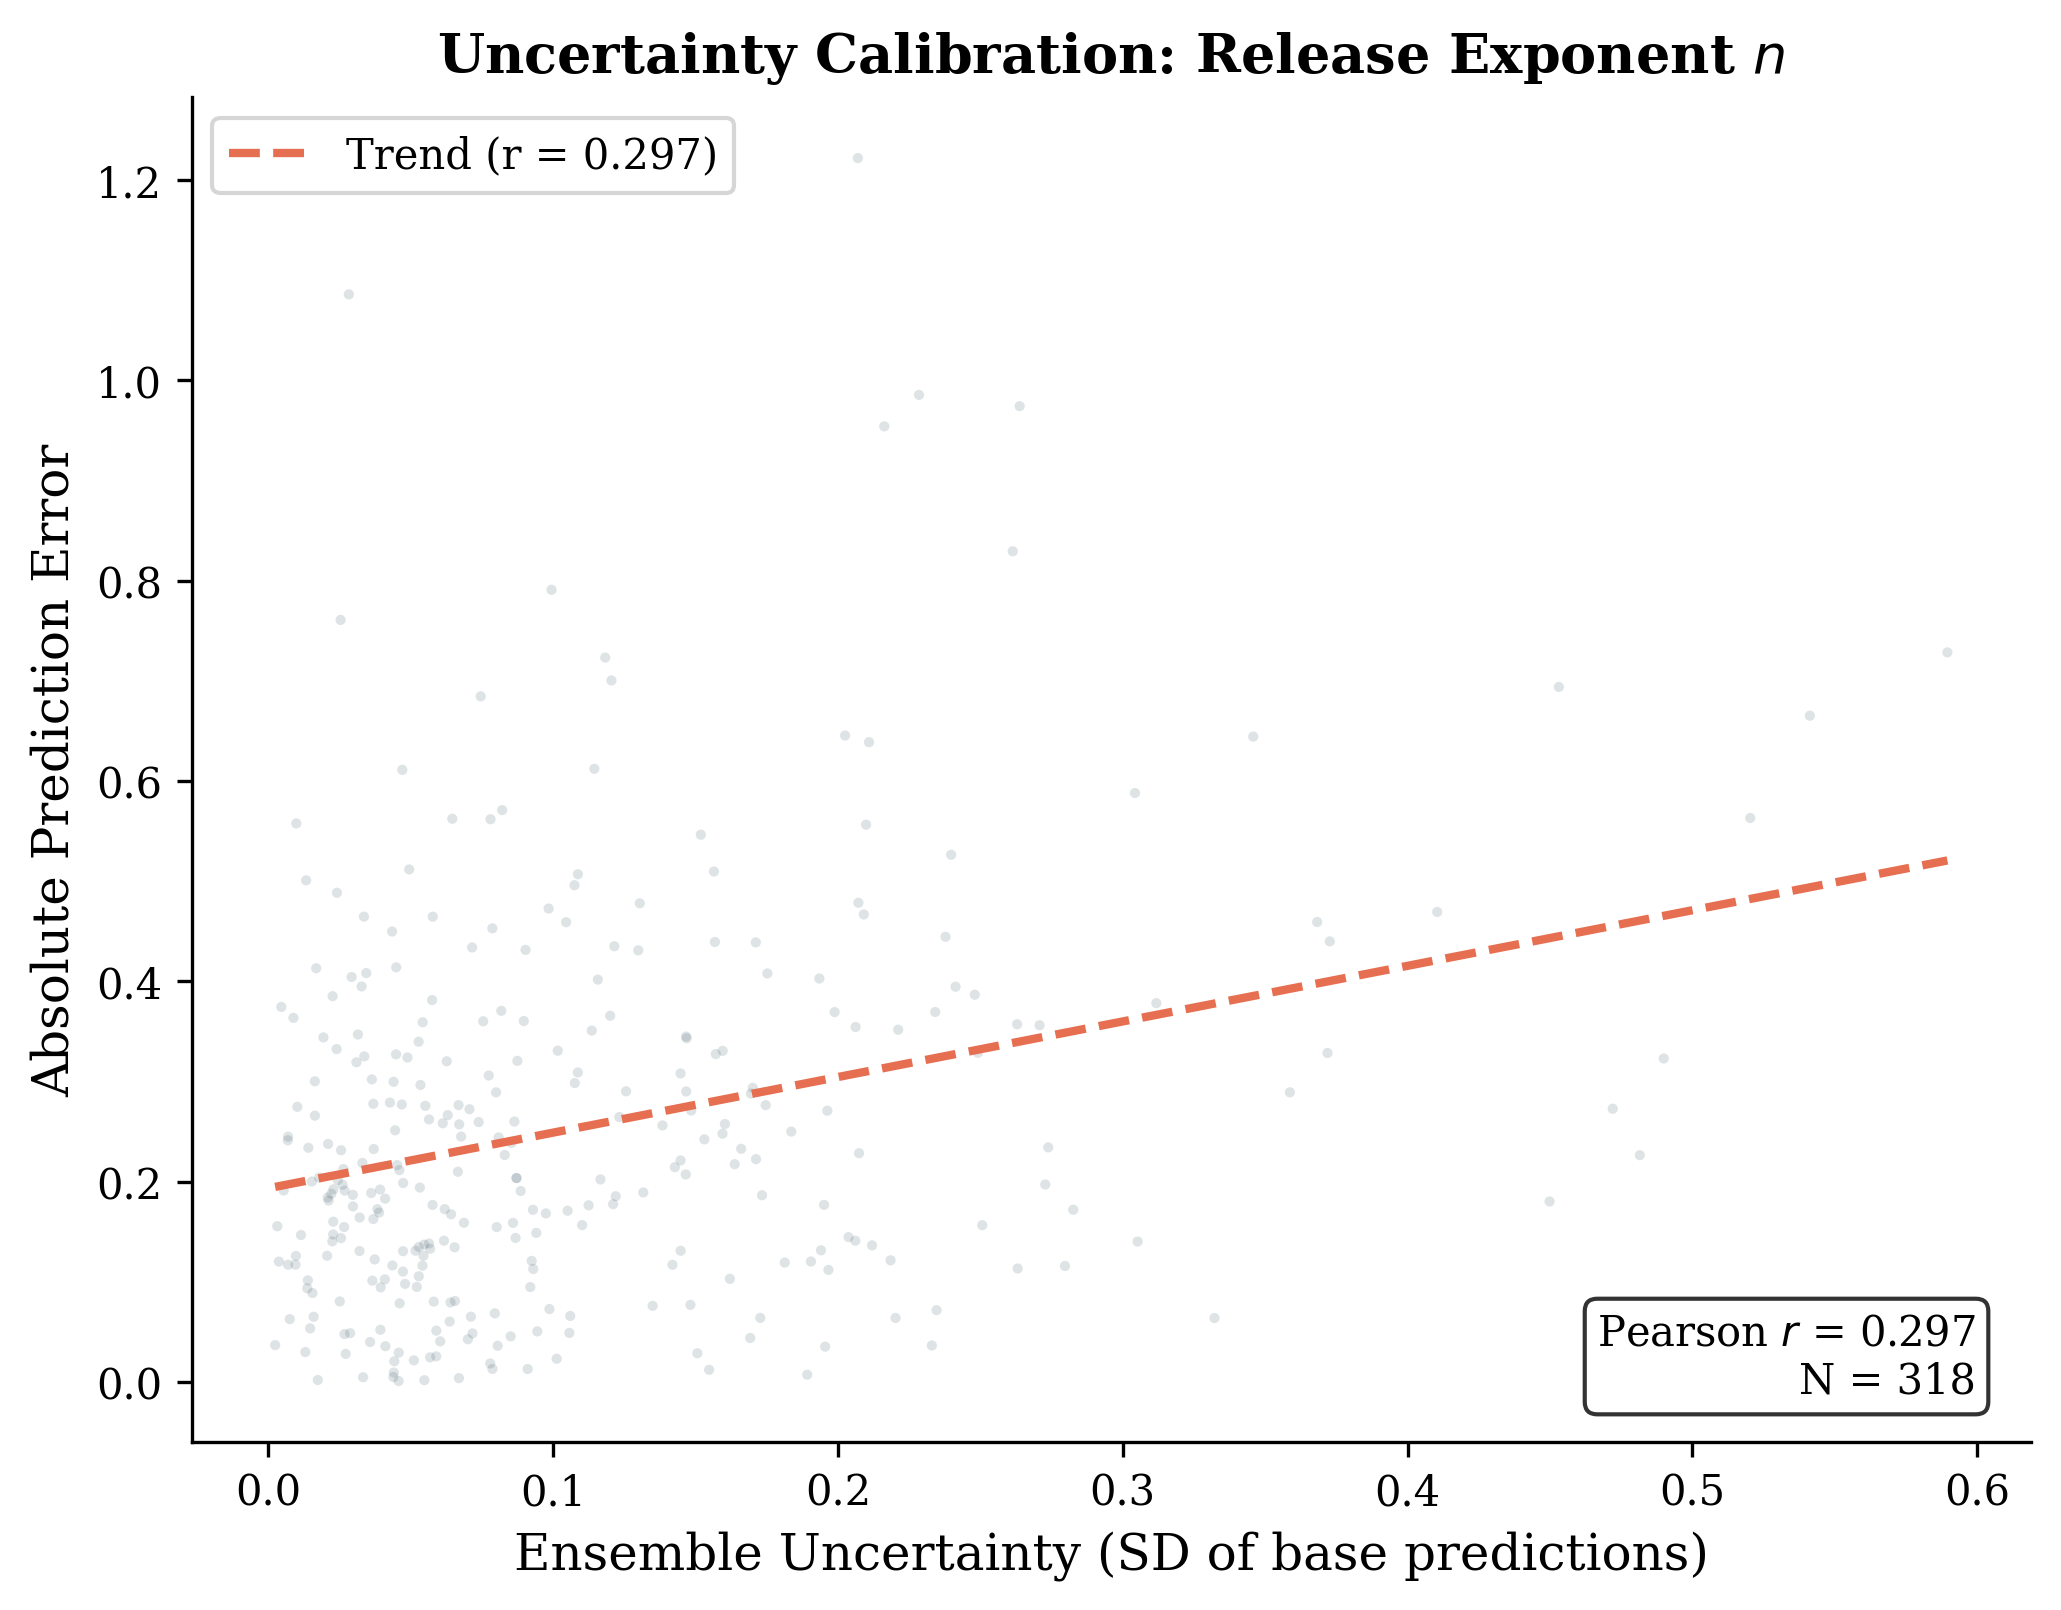
\includegraphics[width=\linewidth]{figures/fig7_uncertainty_calibration}
\caption{Uncertainty calibration for the release exponent $n$: ensemble disagreement versus absolute prediction error.}
\label{fig:uncertainty_plot}
\end{figure}

\FloatBarrier

% ============================================================
% 3.9  LOSO VALIDATION — NEW SECTION
% ============================================================
\subsection{Leave-One-Study-Out Validation}
\label{sec:loso}

To assess the robustness of the grouped cross-validation results and test whether the observed predictive ceiling is an artifact of fold construction, leave-one-study-out (LOSO) validation was performed. In this protocol, each of the 113 unique studies (DOIs) was held out in turn, and the stacked ensemble was trained on the remaining 112 studies and evaluated on the held-out study's formulations. A cross-DOI duplicate check identified only 2 formulation pairs sharing identical features across different DOIs, confirming minimal leakage risk.

LOSO produced substantially lower pooled metrics than grouped 10-fold CV across all three targets (Table~\ref{tab:loso}). For the release exponent $n$, LOSO $R^2 = -0.083$ (MAE = 0.313, RMSE = 0.404), compared to grouped CV $R^2 = 0.347$ (MAE = 0.262, RMSE = 0.332). For $K$, LOSO $R^2 = -0.010$ (MAE = 0.140, RMSE = 0.177), and for \texttt{Burst\_24h}, LOSO $R^2 = -0.180$ (MAE = 0.202, RMSE = 0.245). Under leave-one-study-out validation, all targets yielded negative $R^2$, indicating that models trained on published covariates perform worse than a na\"ive mean predictor when applied to unseen studies. The contrast with within-study grouped cross-validation---where the ensemble recovers meaningful structure ($R^2 = 0.347$ for $n$)---localizes the performance collapse to the between-study variance component. In a random-effects framework, when the majority of outcome variance is attributable to study-level random intercepts (ICC $\approx 0.66$--0.68 for $n$ and $K$; Section~\ref{sec:loso}), models trained without access to study identity are expected to degrade under LOSO validation, because the dominant variance component lies outside the modeled covariate space.

The gap between LOSO and grouped CV quantifies the magnitude of study-level confounding. Negative pooled $R^2$ across all targets indicates that inter-study variability---driven by latent, unreported process variables (solvent removal rate, homogenization energy, internal porosity)---dominates the learnable signal. The negative $R^2$ is therefore a quantitative fingerprint of the information ceiling imposed by current reporting practices.

% ============================================================
% TABLE 8: LOSO vs Grouped CV
% ============================================================

\begin{table}[H]
\centering
\caption{Comparison of grouped 10-fold CV and leave-one-study-out (LOSO) validation.}
\label{tab:loso}
\begin{tabular}{lcccccc}
\toprule
 & \multicolumn{3}{c}{Grouped 10-fold CV} & \multicolumn{3}{c}{LOSO} \\
\cmidrule(lr){2-4} \cmidrule(lr){5-7}
Target & $R^2$ & MAE & RMSE & $R^2$ & MAE & RMSE \\
\midrule
Peppas\_n & 0.347 & 0.262 & 0.332 & $-0.083$ & 0.313 & 0.404 \\
Peppas\_K & 0.174 & 0.138 & 0.171 & $-0.010$ & 0.140 & 0.177 \\
Burst\_24h & 0.026 & 0.160 & 0.205 & $-0.180$ & 0.202 & 0.245 \\
\bottomrule
\end{tabular}
\end{table}

\begin{figure}[H]
\centering
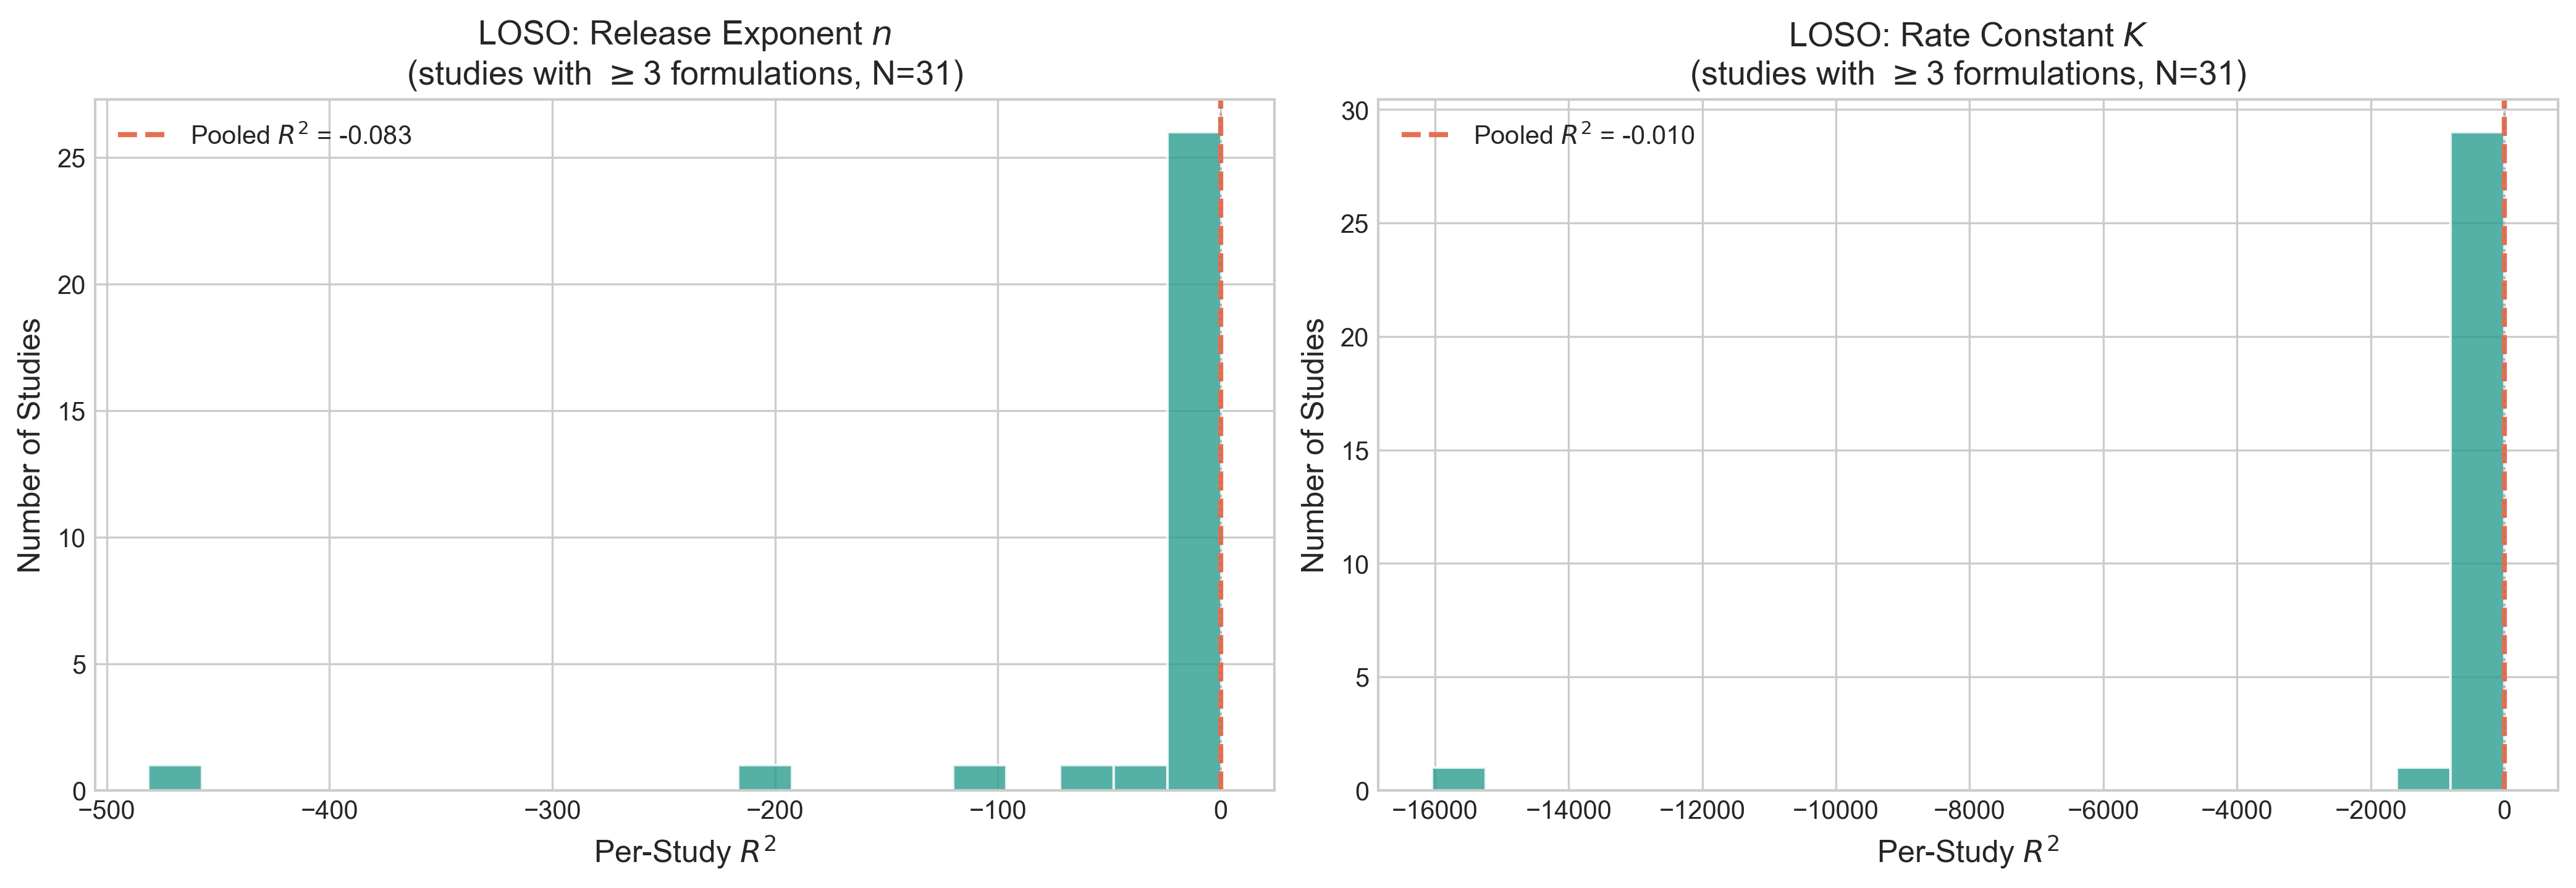
\includegraphics[width=\linewidth]{figures/fig8_loso_distribution}
\caption{Distribution of per-study $R^2$ under LOSO validation for the release exponent $n$ and rate constant $K$. Only studies contributing $\geq 3$ formulations to the held-out set are included. The pooled LOSO $R^2$ is marked as a dashed vertical line.}
\label{fig:loso_dist}
\end{figure}

\paragraph{Variance decomposition by study identity.}
To quantify the fraction of total variance attributable to study-level effects, a one-way random-effects analysis (ICC-1) was performed on the 57 studies contributing $\geq 2$ formulations (265 formulations; Table~\ref{tab:icc}). For the release exponent $n$, 67.5\% of the total variance was attributable to study identity (ICC = 0.675, $F(56, 208) = 10.55$, $p < 0.001$). For $K$, the between-study fraction was 66.0\% (ICC = 0.660), and for \texttt{Burst\_24h}, 45.9\% (ICC = 0.459); all $F$-tests were significant at $p < 0.001$. These estimates confirm that the majority of the variance in fitted release parameters originates between laboratories rather than between formulations within the same study---precisely the variance component that LOSO validation exposes and that unreported process variables are expected to generate. The lower ICC for \texttt{Burst\_24h} (0.459 vs.\ $\sim$0.67 for $n$ and $K$) is consistent with the known sensitivity of early-time release to surface microstructure and batch-level variability, which introduce substantial within-study variance even under nominally consistent protocols.

% ============================================================
% TABLE: ICC Variance Decomposition
% ============================================================

\begin{table}[H]
\centering
\caption{Variance decomposition of release parameters by study identity (ICC-1, one-way random effects model). Only studies contributing $\geq 2$ formulations are included.}
\label{tab:icc}
\begin{tabular}{lcccccc}
\toprule
Target & $k$ & $N$ & $\sigma^2_{\text{between}}$ & $\sigma^2_{\text{within}}$ & ICC(1) & $F$ ($p$-value) \\
\midrule
Peppas\_n & 57 & 265 & 0.1413 & 0.0680 & \textbf{0.675} & 10.55 ($< 0.001$) \\
Peppas\_K & 57 & 265 & 0.0246 & 0.0127 & \textbf{0.660} & 9.92 ($< 0.001$) \\
Burst\_24h & 57 & 265 & 0.0228 & 0.0268 & \textbf{0.459} & 4.89 ($< 0.001$) \\
\bottomrule
\multicolumn{7}{l}{\footnotesize $k$ = number of studies with $\geq 2$ formulations; $N$ = total formulations in those studies.} \\
\end{tabular}
\end{table}

\FloatBarrier

% ============================================================
% 3.10  REPORTING GAP ANALYSIS — NEW SECTION
% ============================================================
\subsection{Reporting Gap Analysis}
\label{sec:reporting_gaps}

Table~\ref{tab:reporting_gaps} cross-references variable availability with predictive importance and mechanistic relevance. Polymer molecular weight---the dominant predictor (27.7\% importance)---was reported in a standardized form ($M_w$) by 59\% of studies. Many studies instead reported an unspecified ``molecular weight'' value without distinguishing $M_w$ from $M_n$, and a small fraction reported only $M_n$. Because these reporting categories overlap across studies (some report both $M_w$ and an unspecified MW elsewhere), we summarize availability at the formulation level: after harmonization (priority: $M_w > M_n >$ unspecified), a usable numeric polymer MW feature could be constructed for 64\% of formulations; the remaining cases required imputation. Critical polymer descriptors---$M_n$ (reported in 5\% of studies) and polydispersity index (PDI, reported in 4\%)---were too sparse to include in the model matrix despite their established roles in controlling chain-end density and molecular weight distribution breadth, both of which influence degradation kinetics and pore formation. Formulation method (O/W, S/O/W, W/O/W) was universally reported but was excluded from the numeric feature matrix to preserve a consistent numerical design space for leverage-based applicability domain calculations; exploratory models incorporating one-hot-encoded method indicators did not materially improve cross-validated performance ($\Delta R^2 < 0.01$ for all targets), suggesting that method effects are largely confounded with the continuous covariates already present.

Below these partially reported variables, Table~\ref{tab:reporting_gaps} lists four mechanistically important process-level variables that are never or almost never quantified in the source literature: internal porosity, solvent removal rate, stirring/homogenization parameters, and polymer end-group chemistry. For end-group chemistry specifically, some information might in principle be recovered from polymer trade names (e.g., the ``H'' suffix in Resomer~RG~502H denotes acid-terminated chains); however, grade-level identifiers were inconsistently reported, and no systematic rescue of end-group data was achievable across the 113 studies compiled here. These variables are known to govern early-time drug release, skin formation, and degradation pathway selection \citep{Fredenberg2011, Makadia2011}, yet their absence from the literature precludes quantitative modeling. The asymmetry between variable importance and variable reporting completeness is striking: the single most important feature (Polymer MW, 27.7\% importance) is available in standardized $M_w$ form for only 59\% of studies, while the mechanistic process variables most likely to resolve the remaining variance---internal porosity, solvent removal rate, stirring energy, end-group chemistry---are reported in 0\% of studies. This pattern directly supports the information-ceiling interpretation: the predictive ceiling is set by the reporting practices of the field rather than by algorithmic limitations.

These findings suggest a concrete set of minimum reporting standards for future PLGA microparticle studies. To enable cross-study predictive modeling, authors should report: (i)~both $M_w$ and $M_n$ of the polymer, determined by gel permeation chromatography, along with PDI; (ii)~polymer end-group chemistry (acid-terminated vs.\ ester-capped); (iii)~solvent removal protocol, including evaporation temperature, duration, and reduced pressure if applicable; (iv)~homogenization energy input (stirring rate in rpm, duration, and probe/impeller type); and (v)~a quantitative measure of internal porosity (e.g., mercury intrusion porosimetry or BET surface area). Adoption of these reporting elements would provide the process-level covariates needed to resolve the inter-study variance that currently dominates the noise floor, and would bring PLGA formulation reporting into closer alignment with Quality by Design (QbD) principles \citep{ICH2009}.

% ============================================================
% TABLE 7: Reporting Gaps
% ============================================================

\begin{table}[H]
\centering
\caption{Reporting gap analysis: variable availability versus predictive importance and mechanistic relevance. Variables below the mid-rule are not reported in the source literature but are known mechanistic drivers of release behavior.}
\label{tab:reporting_gaps}
\small
\begin{tabular}{llccll}
\toprule
Variable & Category & Reported (\%) & Importance (\%) & Mechanistic Role & In Model \\
\midrule
Polymer MW$^{a}$ & Polymer & 64$^{c}$ & 27.7 & Degradation rate, chain mobility & Yes (composite) \\
Polymer $M_w$ & Polymer & 59 & --- & Weight-avg MW; preferred source & Yes$^{b}$ \\
Polymer $M_n$ & Polymer & 5 & --- & Number-avg MW; chain-end density & No (94\% missing) \\
PDI & Polymer & 4 & --- & MW distribution breadth & No (96\% missing) \\
LA:GA ratio & Polymer & 100 & 6.1 & Hydrophilicity, degradation rate & Yes \\
Particle size & Formulation & 100 & 4.8 & Surface area, diffusion path & Yes \\
Drug loading & Formulation & 100 & 3.5 & Drug--polymer interaction & Yes \\
Encapsulation eff. & Formulation & 100 & 5.3 & Process efficiency proxy & Yes \\
Formulation method & Process & 100 & --- & Microstructure determinant & No (categorical) \\
Drug MW & Drug & 100 & 13.0 & Diffusivity, solubility & Yes (RDKit) \\
MolLogP & Drug & 100 & 11.8 & Lipophilicity, partitioning & Yes (RDKit) \\
\midrule
Internal porosity & Microstructure & 0 & --- & Pore-mediated diffusion & No (not reported) \\
Solvent removal rate & Process & 0 & --- & Skin formation, porosity & No (not reported) \\
Stirring/homogenization & Process & 0 & --- & Droplet size, uniformity & No (not reported) \\
End-group chemistry & Polymer & 0 & --- & Acidic vs ester end; degradation & No (not reported) \\
\bottomrule
\multicolumn{6}{l}{\footnotesize $^{a}$Composite of $M_w$, $M_n$, or unspecified MW (priority: $M_w > M_n >$ unspecified).} \\
\multicolumn{6}{l}{\footnotesize $^{b}$Contributes to composite Polymer MW when available.} \\
\multicolumn{6}{l}{\footnotesize $^{c}$Formulation-level availability after harmonization; study-level reporting categories are non-mutually exclusive.} \\
\end{tabular}
\end{table}

\FloatBarrier

% ============================================================
% LIMITATIONS (standalone section)
% ============================================================
\section{Limitations}
\label{sec:limitations}

Several limitations of this study should be acknowledged. First, release data were extracted from published figures using WebPlotDigitizer, introducing digitization noise on the order of a few percent of the ordinate value per point; this uncertainty propagates into the fitted Korsmeyer--Peppas parameters but is unlikely to account for the magnitude of inter-study variance observed. Second, protocol heterogeneity across source studies---including differences in dissolution medium (PBS vs.\ SIF), sink conditions, agitation method, and sampling frequency---represents a confound that cannot be fully disentangled from the compositional variables modeled here. Third, the attribution of the LOSO performance collapse to ``unreported process variables'' is a mechanistic interpretation supported by the reporting-gap analysis but not a proven causal relationship; unmeasured drug--polymer interactions or batch-to-batch PLGA variability may also contribute. Fourth, burst release is notoriously sensitive to surface-level microstructure---surface porosity, skin thickness, adsorbed drug layers---features that are almost never characterized in the source literature, making the negative LOSO $R^2$ for \texttt{Burst\_24h} ($-0.180$) particularly expected. Finally, the dataset is restricted to microparticles produced by emulsion-based methods and may not generalize to spray-dried, electrosprayed, or microfluidic formulations.
